Azure SQL Data Warehouse is a cloud-based data warehouse that uses Massive Parallel Processing (MPP).

MPP allows a high number of processors, even located on different machines, to work on different parts of the same task simultaneously.

Thanks to MPP it is possible to run complex queries across petabytes of data.

\subsubsection{Data storage}
    The data warehouse data is stored separately on Azure Storage.
    
    The data itself is sharded into several \textbf{distributions} across different nodes, to improve performance.

\subsubsection{Massive Parallel Processing}
    Massive Parallel Processing is managed in Azure SQL Data Warehouse by a node-based architecture \cite{bib:azure:dwh:mpp}, as shown in Figure \ref{fig:azure:dwh:mpp}.
    
    \begin{figure}
        \centering
        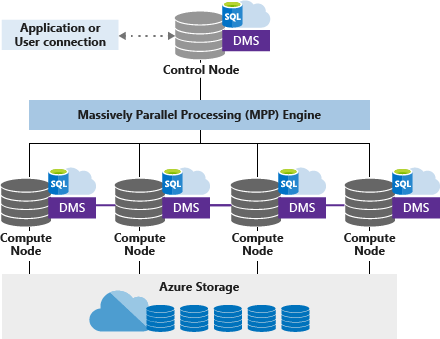
\includegraphics[width=.6\textwidth]{res/azure/dwh/mpp.png}
        \caption{Azure SQL Data Warehouse MPP architecture.}
        \label{fig:azure:dwh:mpp}
    \end{figure}
    
    Queries are sent to the Control node, which optimizes the work for parallel processing, before sending it to Compute nodes, which execute it.
    
    \paragraph{Control node}
        The control node can be defined as the brain of the data warehouse.
        It receives commands and runs a MPP engine, which optimizes and coordinates the work.
        
        Queries are split into 60 smaller queries\footnote{
            This value appears to be fixed and independent from which the query executed \cite{bib:azure:dwh:mpp}.
        } which can all be run in parallel.
        
        The smaller queries are then assigned to a number of Compute nodes, which execute them.
        
        Each smaller query is executed on a single data distribution.
        
    \paragraph{Compute nodes}
        A compute node is a working unit which executes queries received by the Control node.
        
        An Azure SQL Data Warehouse can have up to 60 compute nodes.
        Depending on how many nodes are available to the system\footnote{
            Their number depends on the chosen plan tier. A higher number of compute nodes comports an higher subscription cost.
        }, the Control node assigns them from 1 to 60 distributions.
        
        For example, if there are 60 nodes available each one will have to compute a single task, whereas if only a single node is available it will have to execute all 60 tasks.

\subsubsection{Limitations}
    MPP allows a low number of parallel queries, which are a fundamental requirement, given that several users will be working the data warehouse at the same time.
    
    Azure SQL data warehouse offers different capacity plan, with different costs and computational power.
    The plan currently chosen by Reply allows up to 12 queries in parallel, which, although is enough for development, it is much too low for the actual needs of the trading and big data departments combined.
    
    The highest plan tier offers up to 128 queries in parallel at more than ten times the actual cost \cite{bib:azure:databricks:concurrency_limits}.
    Even ignoring the economic effects of this choice, the number of queries offered is still not high enough, which means that the data warehouse might not be able to answer all queries in acceptable times.
    
    The solution to this problem is to create a replica of a portion of the data warehouse and to perform the most computationally demanding queries there.
    These replicas will reside on Azure Analysis Services.
    